\documentclass{beamer}

% This file is a solution template for:

% - Talk at a conference/colloquium.
% - Talk length is about 20min.
% - Style is ornate.



% Copyright 2004 by Till Tantau <tantau@users.sourceforge.net>.
%
% In principle, this file can be redistributed and/or modified under
% the terms of the GNU Public License, version 2.
%
% However, this file is supposed to be a template to be modified
% for your own needs. For this reason, if you use this file as a
% template and not specifically distribute it as part of a another
% package/program, I grant the extra permission to freely copy and
% modify this file as you see fit and even to delete this copyright
% notice. 


\mode<presentation>
{
  \usetheme{Madrid}
  % or ...

  \setbeamercovered{transparent}
  % or whatever (possibly just delete it)
}


\usepackage{listings}
\usepackage[english]{babel}

% or whatever

\usepackage[latin1]{inputenc}
% or whatever

\usepackage{times}
\usepackage[T1]{fontenc}
% Or whatever. Note that the encoding and the font should match. If T1
% does not look nice, try deleting the line with the fontenc.


%signals, used in Ingo's figures
\newcommand{\signal}[1]{$\overrightarrow{#1}$}

\graphicspath{{../report/figures/}{figures/}}

% grey for the listings


% settings for the listings
\lstset{language=Haskell,
  linewidth=.9\linewidth,
  stringstyle=\ttfamily,
  basicstyle=\scriptsize\ttfamily,
  frame=lines,
  frameround=ffff,
  backgroundcolor=\color[rgb]{.9,.9,1}}


\title%[Short Paper Title]  (optional, use only with long paper titles)
{Hardware Synthesis in ForSyDe}

\subtitle{The design and implementation of a\\ ForSyDe-to-VHDL Haskell-embedded compiler}

\author[A.Acosta] % (optional, use only with lots of authors)
{Alfonso Acosta\\
\footnotesize \href{mailto:alfonso.acosta@gmail.com}{\nolinkurl{alfonso.acosta@gmail.com}}}

% - Give the names in the same order as the appear in the paper.
% - Use the \inst{?} command only if the authors have different
%   affiliation.

\institute[KTH] % (optional, but mostly needed)
{Master's Thesis Defence\\ICT/ECS\\Royal Institute of Technology, Stockholm}
% - Use the \inst command only if there are several affiliations.
% - Keep it simple, no one is interested in your street address.

\date%[CFP 2003] % (optional, should be abbreviation of conference name)
{June 5th, 2007}
% - Either use conference name or its abbreviation.
% - Not really informative to the audience, more for people (including
%   yourself) who are reading the slides online

\subject{Compilers}
% This is only inserted into the PDF information catalog. Can be left
% out. 



% If you have a file called "university-logo-filename.xxx", where xxx
% is a graphic format that can be processed by latex or pdflatex,
% resp., then you can add a logo as follows:

\pgfdeclareimage[height=0.5cm]{university-logo}{kth_cmyk}
\logo{\pgfuseimage{university-logo}}



% Delete this, if you do not want the table of contents to pop up at
% the beginning of each subsection:
\AtBeginSubsection[]
{
  \begin{frame}<beamer>
    \frametitle{Outline}
    \tableofcontents[currentsection,currentsubsection]
  \end{frame}
}

\AtBeginSection[]
{
  \begin{frame}<beamer>
    \frametitle{Outline}
    \tableofcontents[currentsection]
  \end{frame}
}


% If you wish to uncover everything in a step-wise fashion, uncomment
% the following command: 

\beamerdefaultoverlayspecification{<+->}


\begin{document}

\begin{frame}
  \titlepage
\end{frame}

\begin{frame}
  \frametitle{Outline}
  \tableofcontents[pausesections]
  % You might wish to add the option [pausesections]
\end{frame}


% Structuring a talk is a difficult task and the following structure
% may not be suitable. Here are some rules that apply for this
% solution: 

% - Exactly two or three sections (other than the summary).
% - At *most* three subsections per section.
% - Talk about 30s to 2min per frame. So there should be between about
%   15 and 30 frames, all told.

% - A conference audience is likely to know very little of what you
%   are going to talk about. So *simplify*!
% - In a 20min talk, getting the main ideas across is hard
%   enough. Leave out details, even if it means being less precise than
%   you think necessary.
% - If you omit details that are vital to the proof/implementation,
%   just say so once. Everybody will be happy with that.

\beamerdefaultoverlayspecification{}
\section{Introduction to ForSyDe}
\begin{frame}
  \frametitle{Introduction to ForSyDe}
  %\framesubtitle{Subtitles are optional.}
  % - A title should summarize the slide in an understandable fashion
  %   for anyone how does not follow everything on the slide itself.

  \begin{itemize}
  \item
    ForSyDe: \textit{Formal System Design}
    \begin{itemize}
    \item System Design methodology
    \end{itemize} 
  \item
    Goal: high level of abstraction in system design
    \pause
  \item
    Initial scope: Synchronous Systems
    \begin{itemize}
      \item Synchronous Hardware in particular.
    \end{itemize}
    \pause
  \item
    Key concepts
    \begin{itemize}
    \item Signal: \hspace{.5cm} $\overrightarrow{s} = \ll v_0,v_1,v_2,\dots \gg$
      \pause
        \vspace{.3cm}
      \item Process:\hspace{.4cm}
        \visible<4->{ % \uncover doesn't work because the pdf background 
                      % can't be transparent
          \begin{minipage}{2cm}
            \input{../report/figures/Process.pdf_t}
          \end{minipage}
        }
    \end{itemize}
  \end{itemize}
\end{frame}
\beamerdefaultoverlayspecification{<+->}

\begin{frame}
  \frametitle{Introduction to ForSyDe}
  \framesubtitle{Simplified Design Flow}
  % - A title should summarize the slide in an understandable fashion
  %   for anyone how does not follow everything on the slide itself.
  \beamerdefaultoverlayspecification{}
  \only<1>{
    \centering
    \pgfimage[height=6cm]{figures/ForSyDe}
  }
  \begin{columns}
    \column{.62\textwidth}
    \only<2>{
      \begin{enumerate}[0)]
      \item The designer creates the \textbf{specification model} as a
        network of processes.
        
        \vspace{.5cm}
        
        \hspace{.5cm}\input{../report/figures/ConcurrentProcesses.pdf_t}
      \end{enumerate}
    }
    \only<3>{
      \begin{enumerate}[1)]
      \item \textbf{Transformational refinement}
        \begin{itemize}
        \item The \textbf{specification model}
          is transformed into a lower-level \textbf{implementation model}
        \item Bridges the abstraction gap
        \item Relies on the formal foundations of ForSyDe
        \item Not yet implemented
        \end{itemize}
      \end{enumerate}
    }
    \only<4>{
      \begin{enumerate}[2)]
      \item \textbf{Implementation Mapping}
        \begin{itemize}
        \item Transforms the \textbf{implementation model} into
          an architecture-specific implementation
          \begin{itemize}
          \item Software: C, C++ $\dots$
          \item Hardware: VHDL, Verilog $\dots$
          \end{itemize}
        \item \alert{{\large Goal of this thesis}:\\ mapping to VHDL}
        \item The lack of automatization of of (1) entails
          working with the \textbf{specification model}
        \end{itemize}
      \end{enumerate}
    }
    \column{.38\textwidth}
    \pgfimage<2->[height=6cm]{figures/ForSyDe}
  \end{columns}
\end{frame}

\beamerdefaultoverlayspecification{<+->}

\begin{frame}[fragile]
  \frametitle{Introduction to ForSyDe}
  \framesubtitle{ForSyDe's Implementation.}
  % - A title should summarize the slide in an understandable fashion
  %   for anyone how does not follow everything on the slide itself.

  \begin{itemize}
  \item The specification model is expressed in a Haskell-embedded 
    DSL (\textit{Domain Specific Language})
  \pause
  \item Signals modelled as streams of values
    \begin{lstlisting}
      data Signal a = NullS | a :- Signal a
    \end{lstlisting}
  \pause
  \item Sample process constructor: 
    \hspace{.3cm}
    \visible<3->{
    \begin{minipage}{2cm}
    \input{../report/figures/mapSY.pdf_t}
    \end{minipage}
    }
    \begin{lstlisting}
      mapSY :: (a -> b) -> Signal a -> Signal b
      mapSY _ NullS	= NullS
      mapSY f (x:-xs)	= f x :- (mapSY f xs)
    \end{lstlisting}

  \end{itemize}
\end{frame}



\begin{frame}[fragile]
  \frametitle{Introduction to ForSyDe}
  \framesubtitle{$\mathit{plus1}$: A trivial system}
  % - A title should summarize the slide in an understandable fashion
  %   for anyone how does not follow everything on the slide itself.
  \begin{itemize}
    \item $\mathit{plus1}$:  adds 1 to its input signal and forwards it.
      \pause
      \visible<2->{
        \begin{center}
          \hspace{-2cm}\input{../report/figures/plus1.pdf_t}
        \end{center}
      }
      \item Implemented as
      \begin{lstlisting}
        plus1 :: Num a => Signal a -> Signal a
        plus1 = mapSY (+1)
      \end{lstlisting}
  \end{itemize}
\end{frame}


\section{Compiler Design Alternatives}

\beamerdefaultoverlayspecification{}
\begin{frame}
  \frametitle{Compiler Design Alternatives}
  % - A title should summarize the slide in an understandable fashion
  %   for anyone how does not follow everything on the slide itself.
  \begin{enumerate}[(1)]
    
    \item \textbf{Traditional stand-alone compiler}
      \begin{itemize}  
      \item Code a Haskell-to-VHDL compiler from scratch
      \item GHC: 150.000 lines of code (72 years of dedication for one person)
      \end{itemize}
      \pause
    \item \textbf{Customizing an existing compiler}
      \begin{itemize}
      \item Incorporate a new backend to an existing compiler
      \item GHC code generation subtree: 5.000 lines, 14 months
      \end{itemize}
      \pause
    \item Using an \textbf{embedded compilation model}
      \begin{itemize}
      \item The compiler is included in the language library.
      \item Signals keep track of the structure of the circuit.
      \item Used successfully by Lava, a Haskell-embedded HDL.
    \end{itemize}
  \end{enumerate}
\end{frame}


\subsection{Why an Embedded Compiler?}


\begin{frame}
  \frametitle{Why an Embedded Compiler?}
  % - A title should summarize the slide in an understandable fashion
  %   for anyone how does not follow everything on the slide itself.
  \begin{itemize}
    \item \textbf{Realistic}
      \begin{itemize}
        \item Suits the time and man-power limitations of a thesis
      \end{itemize}
      \pause
    \item \textbf{Saves unnecessary effort}
      \begin{itemize}
      \item The goal is to translate the system structure, not 
        any arbitrary Haskell program
      \end{itemize}
      \pause
    \item \textbf{Previous success} 
      \begin{itemize}
        \item Used by the Lava system.
      \end{itemize}
      \pause
    \item \textbf{Maintainable}
      \begin{itemize}
        \item The compiler is packed with ForSyDe's Library.
      \end{itemize}
      \pause
    \item \textbf{Independent of third-party tools}
      \begin{itemize}
        \item No risk of getting outdated due to external design changes
      \end{itemize}
      \pause
    \item \textbf{Drawback}: The compiler has the limitations of every
      other library
      \begin{itemize}
      \item There is no access to the AST of the source-code.
      \end{itemize}

    \end{itemize}
\end{frame}


\section{Changes to Lava's Model}
\subsection{Lava vs ForSyDe}

\begin{frame}
  \frametitle{Lava vs ForSyDe}
  % - A title should summarize the slide in an understandable fashion
  %   for anyone how does not follow everything on the slide itself.
  \begin{itemize}
    \item It was decided to use Lava's model.
    \item However, differences between Lava and ForSyDe made impossible to
      simply replicate Lava's model:
    \end{itemize}
      \begin{enumerate}[1)]
      \item ForSyDe already defines a \texttt{Signal} type totally
        different to Lava's \texttt{Signal}.
      \pause
      \item ForSyDe is more behavioural than Lava.
        \begin{itemize}
          \item Lava is purely structural and does not have the equivalent
            of higher order process constructors.
        \end{itemize}
        \pause
      \item ForSyDe's \texttt{Signal} type is polymorphic
      \begin{itemize}
      \item Signals in Lava are supposed to be polymorphic but in
        practice only \texttt{Int} and \texttt{Bool} signals are
        allowed (gates are monomorphic).
        \end{itemize}
      \end{enumerate}
\end{frame}

\beamerdefaultoverlayspecification{<+->}
\subsection{\texttt{HDSignal}: the Hardware Description Signal}

\begin{frame}[fragile]
  \frametitle{\texttt{HDSignal}}
  \framesubtitle{The Hardware Description Signal}
  % - A title should summarize the slide in an understandable fashion
  %   for anyone how does not follow everything on the slide itself.
  \begin{itemize}
    
  \item The embedded compilation model requires storing the structure of the
    circuit in order to process it
    \begin{itemize}
    \item A method called \textit{Observable Sharing} is used in Lava to
      represent the circuit within the signal type.
      \pause
      \begin{itemize}
      \item allows to identify
        cycles in the netlist without losing the semantic power of recursive
        equations.
      \end{itemize}
    \end{itemize}
    \pause
  \item A new signal was introduced for that purpose: \texttt{HDSignal}
    \begin{itemize}
    \item \texttt{HDSignal} keeps track of the circuit structure through
      \textit{Observable Sharing}.
    \item Modifying the original \texttt{Signal} would had caused regressions.
    \end{itemize}
    \pause
  \item Changes caused in $\mathit{plus1}$
\pause
\begin{overprint}
  \onslide<1-5>
\begin{lstlisting}
  mapSY :: (a -> b) -> Signal a -> Signal b
\end{lstlisting}
\begin{lstlisting}
  plus1 :: Num a => Signal a -> Signal a
  plus1 = mapSY (+1)
\end{lstlisting}
\onslide<6>
\begin{lstlisting}
  hdMapSY :: (a -> b) -> HDSignal a -> HDSignal b
\end{lstlisting}
\begin{lstlisting}
  plus1 :: Num a => HDSignal a -> HDSignal a
  plus1 = hdMapSY (+1)
\end{lstlisting}

\end{overprint}

    
\end{itemize}  
\end{frame}

\subsection{\texttt{HDFun}: the Hardware Description Function}

\begin{frame}[fragile]
  \frametitle{\texttt{HDFun}}
  \framesubtitle{The Hardware Description Function}
  % - A title should summarize the slide in an understandable fashion
  %   for anyone how does not follow everything on the slide itself.
  \begin{itemize}
    \item \texttt{HDSignal} is not enough to store the
      circuit definition.
      \begin{lstlisting}
        hdMapSY :: (a -> b) -> HDSignal a -> HDSignal b
      \end{lstlisting}
    \item \texttt{(a->b)} does not contain syntax information from which 
      to translate the original function to VHDL.
\pause
    \item Solution: use Template Haskell to store the AST of the original
      function in a new ADT: \texttt{\textbf{HDFun}}.
      \begin{lstlisting}
    hdMapSY :: HDFun (a -> b) -> HDSignal a -> HDSignal b
      \end{lstlisting}
\pause
    \item Changes in $\mathit{plus1}$
\begin{overprint}
  \onslide<1-3>
\begin{lstlisting}
   plus1 :: Num a => HDSignal a -> HDSignal a
   plus1 = hdMapSY (+1)
\end{lstlisting}
\onslide<4>
\begin{lstlisting}
   plus1 :: Num a => HDSignal a -> HDSignal a 
   plus1 = hdMapSY doPlus1
      where doPlus1 = 
              $(mkHDFun [d| doPlus1 :: Num a => a -> a
                            doPlus1 a = a + 1          |])
\end{lstlisting}
\end{overprint}
      
    \end{itemize}  
\end{frame}


\subsection{Controlling Polymorphism: \texttt{HDPrimType}}

\begin{frame}[fragile]
  \frametitle{Controlling Polymorphism}
  \framesubtitle{The \texttt{\textbf{HDPrimType}} type class}
  % - A title should summarize the slide in an understandable fashion
  %   for anyone how does not follow everything on the slide itself.
  \begin{itemize}
    
  \item Apparently, \texttt{hdMapSY} finally has everything required to 
    compile
      \begin{lstlisting}
    hdMapSY :: HDFun (a -> b) -> HDSignal a -> HDSignal b
      \end{lstlisting}
  \pause
\item There is still a problem: it is too generic.
  \begin{itemize}
    \item There is no way to automatically translate every kind of
      signal value to VHDL.
    \end{itemize}
  \pause
  \item Solution: limit the subset of signal values through a class
    constraint: \texttt{\textbf{HDPrimType}}, the \textit{Hardware
      Description Primitine} Type class.
    
\begin{lstlisting}
   hdMapSY :: (HDPrimType a, HDPrimType b) => 
              HDFun (a->b) -> HDSignal a -> HDSignal b
\end{lstlisting}
\pause
\item The types belonging to \texttt{HDPrimType} are the only ones
  suitable to be compiled.
\begin{itemize}  
\item Currently only \texttt{Int} and \texttt{Bool} are supported.
\end{itemize}

\end{itemize}  
\end{frame}

\subsection{Integration with ForSyDe}

\begin{frame}[fragile]
  \frametitle{Integration with ForSyDe}
  % - A title should summarize the slide in an understandable fashion
  %   for anyone how does not follow everything on the slide itself.
  \begin{itemize}
  \item \texttt{mapSY} was renamed to \texttt{hdMapSY} to avoid a
    name-clash but, is there a way to share the same name?
  \pause
  \item Solution: MPTC (\textit{Multiparameter Type Classes})
    \begin{lstlisting}
  class SynchronousM f_a_b signal a b 
        | signal a b -> f_a_b where
   mapSY :: f_a_b -> signal a -> signal b

  instance SynchronousM (a->b) Signal a b where
    mapSY ... -- same definition

  instance (HDPrimType a, HDPrimType b)
    => SynchronousM (HDFun (a->b)) HDSignal a b where
   mapSY = -- hidden details
\end{lstlisting}
\pause
\item Sweet collateral effect: all the derived processes purely based
  in in \texttt{mapSY} work out of the box both for \texttt{Signal} and
  \texttt{HDSignal}
\end{itemize}  
\end{frame}

\section{Improvements to Lava's Model}

\begin{frame}[fragile]
  \frametitle{Improvements to Lava's Model}
  \framesubtitle{Ports}
  % - A title should summarize the slide in an understandable fashion
  %   for anyone how does not follow everything on the slide itself.
  \begin{itemize}
  \item Port: interface between the system and the outside world.
  \item Lava and ForSyDe use tuples to deal with multiple outputs
    \begin{itemize}  
    \item tuples lead to multiple data representations requiring
      to agree on conventions
    \item i.e. {\scriptsize \texttt{(Int, Bool, Int)} \texttt{((Int,
          Bool), Int)} \texttt{(Int, (Bool, Int))}}
    \item Ports treat data uniformly and improve readibility of the code 
    \end{itemize}
  \pause
  \item Ports of $\mathit{plus1}$
\begin{lstlisting}
  plus1In :: InPort
  plus1In = mkInPort 1 [("plus1Input", Int)]

  plus1Out :: OutPort
  plus1Out = mkOutPort 1 [("plus1Output", Int)]
\end{lstlisting}
  \end{itemize}  
\end{frame}


\begin{frame}
  \frametitle{Improvements to Lava's Model}
  \framesubtitle{Circuits, Blocks and Block Instances}
  % - A title should summarize the slide in an understandable fashion
  %   for anyone how does not follow everything on the slide itself.
  \begin{itemize}
    
  \item Circuit, Blocks and Block Instances add hierarchical and
    reusability design support within the compiler.
    
    \hspace{-.5cm}
    \begin{tabular}{c|c|c}
    \includegraphics[height=2.5cm]{figures/Circuit.png}
    &
    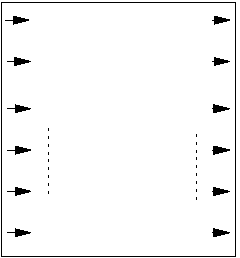
\includegraphics[height=2.5cm]{figures/Block.png}
    &
    \includegraphics[height=2.5cm]{figures/Instance.png}
     \\
     Circuit & Block & Block Instance \\
     \end{tabular}
     
   \item Block: white box. Internals known but isolated from the
     outside world
   \item Block Instance: black box. Connectable to the outside world
     but unkown internals (similar to VHDL \textit{components})
  \end{itemize}  
\end{frame}


\begin{frame}[fragile]
  \frametitle{Improvements to Lava's Model}
  \framesubtitle{Circuits, Blocks and Block Instances (II)}
  % - A title should summarize the slide in an understandable fashion
  %   for anyone how does not follow everything on the slide itself.
  
\begin{itemize}
\item In the case of $\mathit{plus1}$
\item Circuit:
\begin{lstlisting}
   plus1Circ :: InPort -> OutPort
   plus1Circ ip = supplySig  plus1Sig "plus1Output" plus1Out
      where plus1Sig = plugSig "plus1Input" ip hdPlus1
\end{lstlisting}
\pause
\item Block:
\begin{lstlisting}
   plus1Block :: Block
   plus1Block = mkBlock "plus1" plus1In plus1Circ
\end{lstlisting}
\pause
\begin{verbatim}
> writeVHDL plus1Block
Writing VHDL code to plus1.vhd ... done!
\end{verbatim}
\pause
\item Block Instance
\begin{lstlisting}
plus1Ins :: BlockIns
plus1Ins = instantiate plus1Block
\end{lstlisting}
\end{itemize}

\end{frame}

\section{Conclusions and Further Work}

\beamerdefaultoverlayspecification{}
\begin{frame}
  \frametitle{Conclusions}
  % - A title should summarize the slide in an understandable fashion
  %   for anyone how does not follow everything on the slide itself.
  \begin{itemize}
    
  \item As a result of this thesis ForSyDe counts with a fully
    functional VHDL compiler.
  \pause
  \item The compiler provides a research framework
  \pause
  \item Due to the embedded compilation model
    \begin{itemize}
      \item Mainteinable (less than 2000 lines of code)
      \item Easy to distribute
      \item Independent of third-party tools
    \end{itemize}
  \pause
  \item New features integrated with the compiler
    \begin{itemize}
      \item Uniform I/O treatment: \textit{Ports}
      \item Hierarchical designs: \textit{Blocks}+\textit{Block Instances}
    \end{itemize}
    \pause
    \item Limitations
      \begin{itemize}
      \item Not tested thoroughly yet
      \item The types of signal values are limited
      \item \texttt{HDFun}s only support a small Haskell subset
      \item Depends on GHC
      \item Cannot access the source AST without Template Haskell tricks
      \end{itemize}
  \end{itemize}  
\end{frame}



\begin{frame}
  \frametitle{Further work}
  % - A title should summarize the slide in an understandable fashion
  %   for anyone how does not follow everything on the slide itself.
  \begin{itemize}
  \item \textbf{Overcome some limitations of the compiler}
    \begin{itemize}
      \item Add support for new \texttt{HDSignal} values.
      \item Extension of \texttt{HDFun}'s Haskell subset

  \end{itemize}
  \pause
\item \textbf{Development of a test suite}
  \pause
  \item \textbf{Automatization of the \textit{Transformational Design
      Refinement} stage}
  \pause
\item \textbf{Development of \texttt{Block} and \texttt{HDFun}
    combinational libraries}
  \pause
  \item \textbf{Support for other backends than  VHDL}
    \begin{itemize}
      \item Simulation, verification, graphical representation
    \end{itemize}
  \pause
  \item \textbf{Development of a graphical frontend}
    
  
    \end{itemize}  
\end{frame}


\section<presentation>*{Further Reading}

\begin{frame}
  \frametitle<presentation>{Further Reading}
    
%   \begin{thebibliography}{10}
    
%   \beamertemplatebookbibitems
%   % Start with overview books.

%   \bibitem{Author1990}
%     A.~Author.
%     \newblock {\em Handbook of Everything}.
%     \newblock Some Press, 1990.
 
    
%   \beamertemplatearticlebibitems
%   % Followed by interesting articles. Keep the list short. 

%   \bibitem{Someone2000}
%     S.~Someone.
%     \newblock On this and that.
%     \newblock {\em Journal of This and That}, 2(1):50--100,
%     2000.
%   \end{thebibliography}
  
%  \nocite*
%  \bibliography{presentation}
%  \bibliographystyle{unsrt}

\begin{thebibliography}{1}



\bibitem{fons:thesis}
Alfonso Acosta.
\newblock {\em Hardware synthesis in ForSyDe: The design and implementation of a Haskell-embedded ForSyDe-to-VHDL compiler}.
\newblock Master's thesis, Royal Institute of Technology, Sweden, 2007.


\bibitem{forsyde:thesis}
Ingo Sander.
\newblock {\em System Modeling and Design Refinement in ForSyDe}.
\newblock PhD thesis, Royal Institute of Technology, Sweden, 2003.

\bibitem{osharing}
Koen Claessen and David Sands.
\newblock Observable Sharing for functional circuit description.
\newblock In {\em Asian Computing Science Conference}, pages 62--73, 1999.


\bibitem{hydra:th}
John~T. O'Donnell.
\newblock Embedding a Hardware Description Language in Template Haskell.
\newblock In {\em Domain-Specific Program Generation}, pages 143--164, 2003.



\end{thebibliography}


\end{frame}


\end{document}


